\begin{center}
    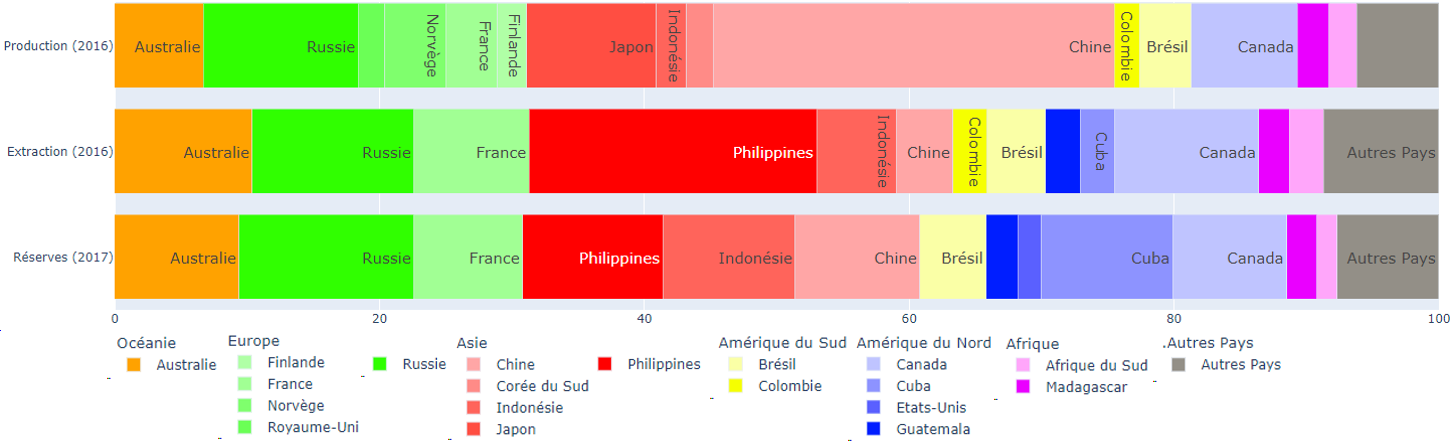
\includegraphics[width=\textwidth]{Illustration métaux/Nickel.png}
\end{center}
\begin{center}
    \textbf{Usages et consommation}
\end{center}
Le nickel est utilisé à 85 \% pour la production d'acier inoxydable ou d'autres alliages. Moins de 7 \% du nickel est actuellement
utilisé pour la production de batterie. Dans le domaine énergétique, le nickel est très critique pour
la géothermie, le stockage d'hydrogène et la fabrication de batteries. Il est modérément critique pour l'énergie
nucléaire, éolienne et solaire à concentration.

\begin{center}
    \textbf{Prospective}
\end{center}
\begin{multicols}{2}
    \begin{center}
        \textit{Total nickel demand by sector and scenario}
    \end{center}
    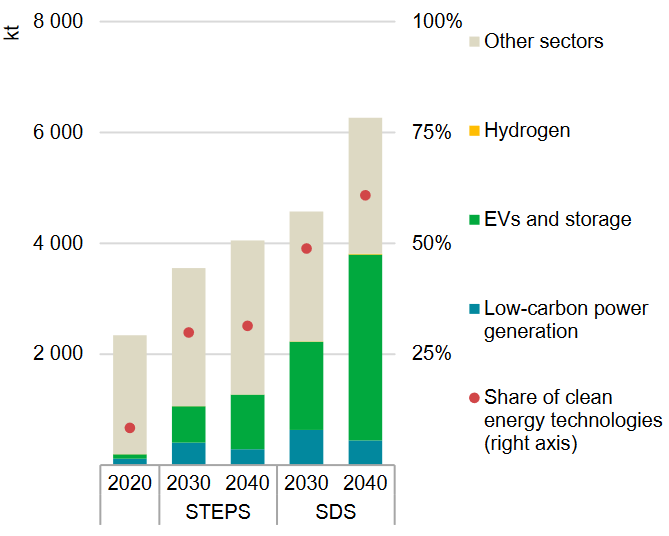
\includegraphics[width=0.45\textwidth]{Illustration métaux/Nickel prospective.PNG}
    \vfill\null
    \columnbreak
    La demande en inox est corrélée au développement économique global. Cependant dans les prochaines années
    la demande en nickel pourrait être fortement stimulée par la fabrication de batterie. Les technologies
    bas-carbone représentent actuellement une faible part de la demande de nickel, mais cette part est amenée à fortement augmenter dans les deux prochaines décennies dépassant 50\% de la demande. Le marché est amené à être bien approvisionné dans les prochaines années, même si des tensions sont possibles avec l'augmentation rapide de la demande en nickel de classe 1 (pur à plus de 99.8\%).
\end{multicols}
\begin{center}
    \textbf{Production et recyclage}
\end{center}
La production minière de nickel a augmenté chaque année en moyenne de 3.93\% de 1945 à 2015. La production minière est de l'ordre de 2 200 kt/an. Le nickel est peu recyclé
en tant que tel, mais les inox et alliages contenant du nickel sont fortement recyclés. Sous toutes ses formes
le taux de recyclage en fin de vie du nickel est d'environ 60\% à l'échelle mondiale. La production minière de La
Nouvelle-Calédonie dont la production est raffinée sur place ou dans la métropole représente 8.7\% de la production mondiale.
\begin{center}
    \textbf{Substituabilité}
\end{center}
Le nickel dans les alliages est difficilement substituable sans contrepartie économique ou technique. L'abondance
et les prix actuels du nickel n'incitent pas à d'avantage de recherches pour la substitution. Des technologies
de batteries avec moins ou pas de nickel sont actuellement matures. 
\begin{center}
    \textbf{Prix}
\end{center}
La volatilité du prix du nickel est modérée. En moyenne à 9 500 US\$/t en 2016, le prix du nickel a atteint un pic très temporaire
à 43 000 US\$/t début 2022 avant la fermeture temporaire du marché pendant l'invasion russe en Ukraine. La valeur du marché de la production métalurgique annuelle de nickel est de l'ordre de 19 G US\$.

\clearpage
\begin{center}
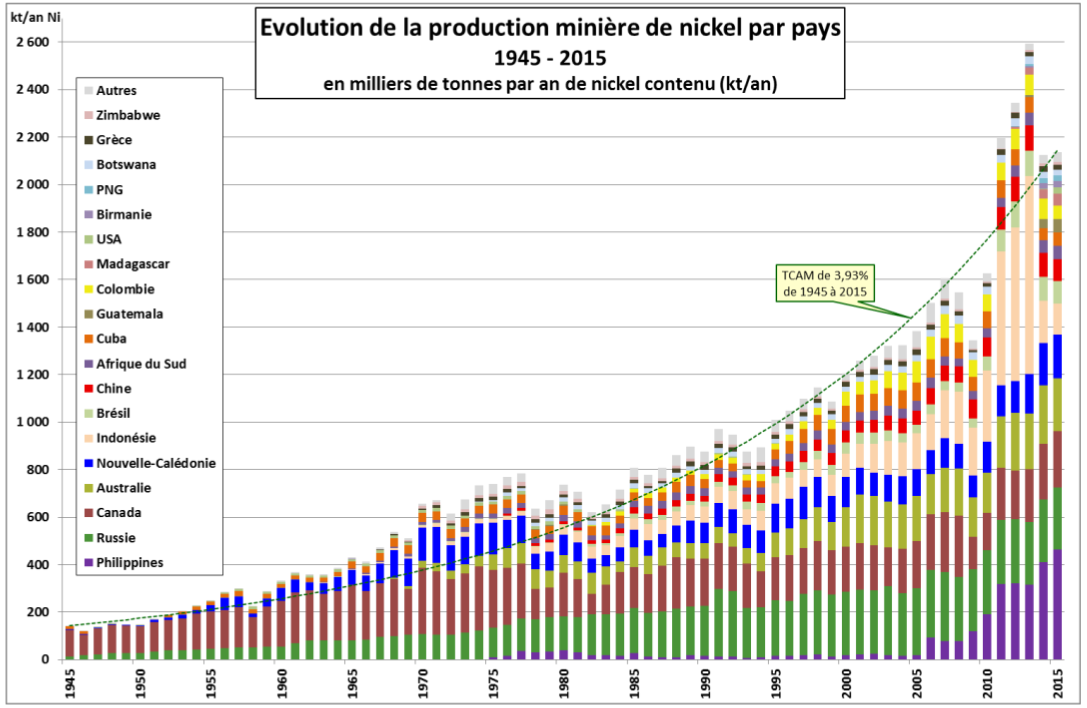
\includegraphics[width=11cm]{Illustration métaux/Dynamique_nickel.png}
\end{center}
\begin{center}
    \textbf{Evènements géopolitiques}
\end{center}
L'Indonésie était le premier producteur minier mondial en 2013 avec 32\% de la production. Le pays est passé au sixième rang en 2015 à la suite de l'embargo décidé sur les exportations de minerai brut entre janvier 2014 et 2017. L'Indonésie a décidé de nouvelles restrictions à partir de 2020 (voir encadré \hyperref[Indonesia]{\textit{L’Indonésie et le nickel : existe-t-il un risque de cartellisation ?}}). 

\begin{multicols}{2}
    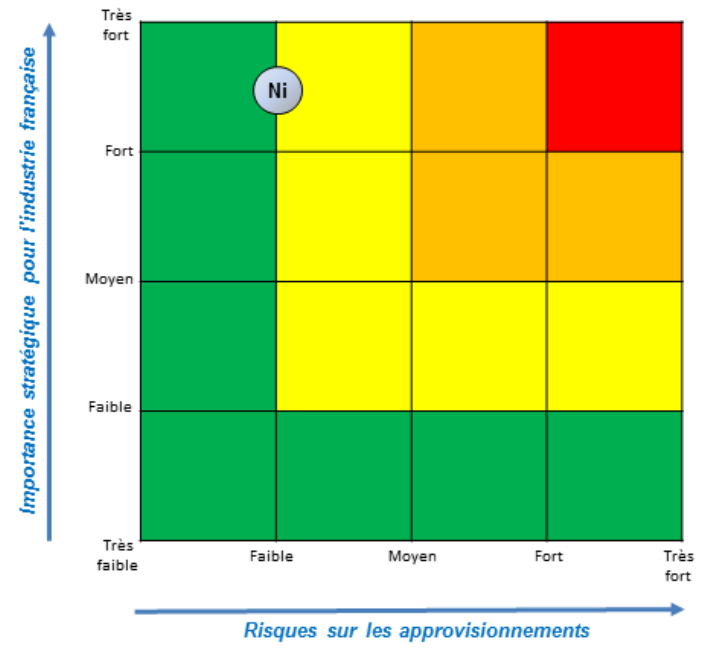
\includegraphics[width=0.35\textwidth]{Illustration métaux/Nickel_criticité.png}
    \begin{center}
    \textbf{Criticité en France}
    \end{center}
    Le risque sur les approvisionnements en nickel est faible en France grâce à la faible concentration
    du marché mondial et grâce à la production en Nouvelle-Calédonie. Il n'empêche que ce métal est peu substituable
    et particulièrement important dans l'économie.
\end{multicols}

\begin{multicols}{2}
    \begin{center}
        \textit{Chaîne d'approvisionnement du nickel}
    \end{center}
    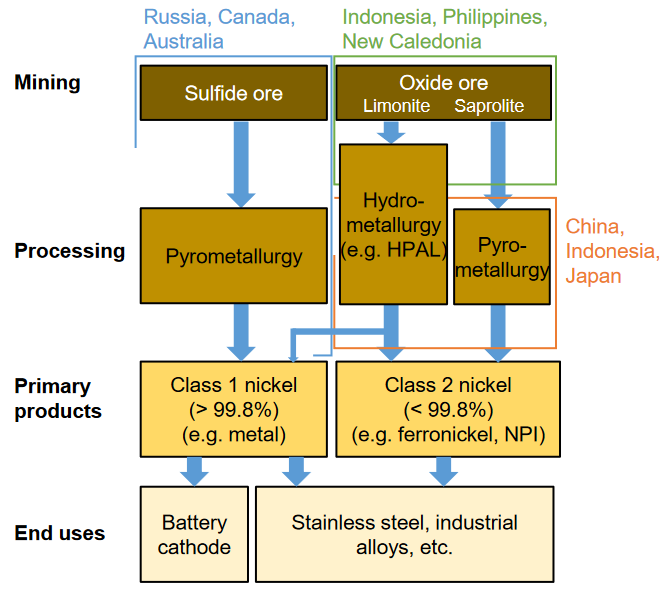
\includegraphics[width=0.45\textwidth]{Illustration métaux/Nickel_supply_chain.PNG}
    \begin{center}
    \textbf{Risques spécifiques}
    \end{center}
    Le nickel raffiné se sépare en deux classes : classe 1 pour une pureté supérieure à 99.8\%, classe 2 sinon.
    Le nickel de classe 1 uniquement peut être utilisé dans les batteries. Seule la production d'un certains type 
    de réserves ("sulfide ore") permet facilement d'acquérir du nickel de classe 1. Le raffinage en classe 1 de
    nickel issu d'autres réserves ("Oxide ore") est actuellement très difficile technologiquement et très onéreux.
\end{multicols}

